\chapter{PIATTAFORMA YUP}
\label{platform_chapter}
In questo Capitolo analizziamo in dettaglio la piattaforma di Yup, in particolare le funzionalità e le principali caratteristiche. Daremo poi una descrizione tecnica del suo protocollo, riportando anche le formule per il calcolo delle ricompense o di altri parametri fondamentali per il suo funzionamento, e del suo cryptoasset. Per concludere, presenteremo lo scopo di questo lavoro di tesi, introducendo le fasi del lavoro (Studio, Download ed Analisi), in cui elencheremo le varie azioni individuate nello Smart Contract.

\section{La piattaforma Yup}
Yup è una dApp prima nel suo genere a puntare su un approccio cross-chain e cross-platform. Di fatto si basa sull'utilizzo dei rispettivi punti di forza di due blockchain, Ethereum per la liquidità e EOS per la scalabilità. La piattaforma consente ai suoi utenti, solitamente definiti come Yupsters all'interno della community,  di valutare l'Internet e le principali piattaforme sociali, ovvero esprimere opinioni su qualsiasi tipo di contenuto, sia esso un tweet, un post, una immagine, un video, un NFT e così via, in qualsiasi sito o piattaforma. Possono inoltre creare delle collezioni personali, in cui inseriscono i loro contenuti preferiti, valutabili dagli altri utenti. 
\\
Le ricompense vengono attribuite esclusivamente tenendo conto dei voti che occorrono dopo quello effettuato dall'utente, in questo modo da un lato si evita che qualcuno voti qualcosa per il semplice fatto che molte altre persone lo abbiano votato, dall'altro viene promosso l'essere i primi a votare un contenuto di qualità. Un approccio di questo tipo porta alla creazione di uno strato di consenso sociale, ovvero dove qualsiasi cosa, individui e contenuti, sono classificati in base al loro valore (sociale).
\\
L'innovatività del progetto risiede nel fatto di non presentarsi come una piattaforma alternativa a quelle già esistenti, bensì come un'integrazione con queste ultime. L'utente deve infatti solamente scaricare l'estensione sul proprio browser per poter iniziare ad utilizzare Yup e non deve abbandonare le sue piattaforme preferite.
\\
\\
Questo obiettivo viene raggiunto tramite l'utilizzo di due componenti, che analizzeremo nel dettaglio nelle sezioni successive, di seguito elencate:

\begin{itemize}
    \item \textbf{Yup protocol:} la componente \textit{software} autonoma e decentralizzata della \textit{dApp} che opera su EOS
    \item \textbf{Yup token:} il \textit{cryptoasset} che viene utilizzato per le ricompense
\end{itemize}

Yup, come detto precedentemente si basa su EOS ed utilizza gli smart contract per gestire i servizi offerti. Nello specifico, dall'elenco presente nella documentazione, sono stati individuati i seguenti smart contracts:

\begin{itemize}
    \item \textbf{yupyupyupyup:} il protocollo vero e proprio (quello principale)
    \item \textbf{token.yup:} relativo allo Yup token
    \item \textbf{lptoken.yup:} relativo al token per i Liquidity Provider (YUP-ETH LP TOKEN)
    \item \textbf{bridge.yup:} relativo al Bridge EOS-ETH
    \item \textbf{lpbridge.yup:} relativo al Bridge di token YUP-ETH LP
\end{itemize}

Di seguito introdurremo in dettaglio i servizi e le caratteristiche di Yup.

\section{Registrazione}
Al momento della scrittura di questa tesi è possibile diventare un utente Yup tramite tre differenti modalità, da cui conseguono differenti vantaggi/svantaggi:

\begin{itemize}
    \item \textbf{Twitter Account}
    \item \textbf{Wallet Connect}
    \item \textbf{Email}
\end{itemize}

Registrandosi tramite \textbf{Wallet Connect} o \textbf{Account Twitter} l'iscrizione sarà immediata, nel caso di Twitter è tuttavia necessario che l'account rispetti due caratteristiche: deve esistere da un certo periodo di tempo e deve possedere almeno 50 followers.
Se invece il metodo prescelto prevede l'utilizzo di una email l'iscrizione sarà completata solo previa revisione e autorizzazione. Le limitazioni poste all'account Twitter e la revisione dell'email sono pratiche introdotte per eliminare, o quantomeno contrastare, l'iscrizione di bot o multi-account sulla piattaforma.
\\
Gli account registrati tramite le prime due modalità partono da un valore di \textbf{Influenza} nettamente superiore rispetto a quelli registrati tramite email (80 invece di 20). Ne consegue la possibilità di avere dei profitti maggiori, fino al 120\% (secondo quanto dichiarato nella frontpage del sito della piattaforma). Da questa differenza ne consegue anche una capacità di voto giornaliera differente, per i vari utenti. Infatti, il numero di voti che un individuo può esprimere è strettamente collegato alla propria influenza. %Daremo una analisi più dettagliata di questo aspetto nella sezione immediatamente successiva.

%\subsection{Mirror Accounts}
All'interno della piattaforma esistono, oltre ad account di utenti reali, che chiameremo \textbf{non-Mirror}, anche account creati e gestiti da Yup che sono relativi ad influencers di Twitter e che chiameremo invece \textbf{Mirror}. Questi ultimi ripetono qualsiasi attività effettuata dal corrispondente account Twitter.
L'obiettivo è dare una rappresentazione dei token guadagnati dai vari influencer in qualità di creatori di contenuti e creare \textit{awareness} per la piattaforma e i possibili guadagni che ne derivano.

\subsection{Voti}
\label{voti_section}
Come accennato precedentemente, gli utenti hanno una capacità di voto giornaliera limitata, che prende il nome di \textbf{Voting Power}. Questa viene resettata ogni 24h, conteggiate a partire dal primo voto espresso con \textbf{Voting Power} piena, e misurata in un range 0\%-100\%. 
I contenuti possono essere valutati in una scala da 1 a 5, dove le valutazioni 1/5 e 2/5 sono da intendere come negative mentre quelle 3/5, 4/5 e 5/5 sono da intendere come positive, secondo una scala non lineare. Ogni rating richiede una differente porzione della propria \textbf{Voting Power} ma ne consegue anche un diverso moltiplicatore delle ricompense (Figura \ref{fig:ratings}).
\begin{figure}[t]
    \centering
    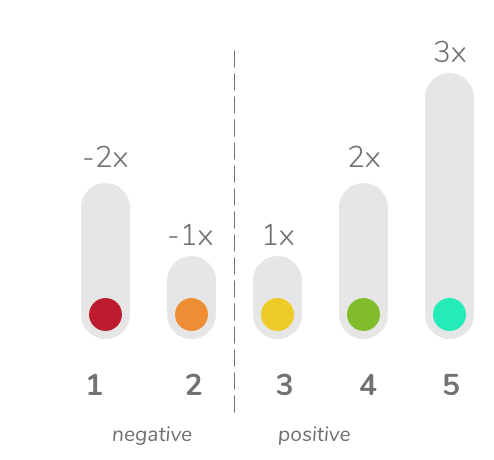
\includegraphics[scale=0.5]{images/ratings.png}
    \caption{Ratings}
    \label{fig:ratings}
\end{figure}
Questo porta l'utente ad esprimere valutazioni "estreme" (1/5 se negativa e 4/5 o 5/5 se positiva) solo per quei contenuti che ritiene veramente validi e valutazioni più moderate per i restanti.

Il numero di voti che un utente può esprimere giornalmente varia con il valore della sua influenza. E' stato infatti possibile osservare come questa determini la porzione di \textbf{Voting Power} che viene sottratta all'utente per uno specifico voto. Approssimativamente nel seguente modo:

\begin{itemize}
    \item \textbf{Nuovi Utenti:}
    \begin{itemize}
        \item 3/5 o 2/5 $\approx$ 20 voti
    \end{itemize}
    \begin{itemize}
        \item 4/5 o 1/5 $\approx$ 5 voti
    \end{itemize}
    \begin{itemize}
        \item 5/5 $\approx$ 2-3 voti
    \end{itemize}
    \item \textbf{Utenti Veterani (Influenza $\geq 90$):}
    \begin{itemize}
        \item 3/5 o 2/5 $\approx$ 40 voti
    \end{itemize}
    \begin{itemize}
        \item 4/5 o 1/5 $\approx$ 10 voti
    \end{itemize}
    \begin{itemize}
        \item 5/5 $\approx$ 4 voti
    \end{itemize}
\end{itemize}
% corretto commento di Andrea

Il voto espresso può successivamente essere modificato, con la variazione del rating espresso, o anche eliminato completamente. Nel primo caso verrà effettuato un aggiustamento della \textbf{Voting Power}, ridotta se il nuovo rating è più estremo del precedente, aumentata se meno estremo, nel secondo caso, la \textbf{Voting Power} viene completamente rimborsata. Da questo consegue la possibilità per gli utenti di cambiare le opinioni espresse nel tempo. Tuttavia alcuni utenti potrebbe abusare questa funzionalità eliminando o modificando propri voti per cui hanno già ricevuto le ricompense, per esempio relativi a post di Twitter sufficientemente vecchi e che quindi difficilmente riceveranno ulteriori voti, con lo scopo di ottenere un rimborso di Voting Power e poter quindi effettuare più voti nell'arco di una giornata. Il problema viene solo parzialmente arginato dal fatto che il numero di azioni che un utente può effettuare in una giornata è limitato. 
% corretto commento di Andrea

L'utente può inoltre scegliere tra tre categorie, prescelte dal sistema e che variano in base a piattaforma/tipo di contenuto, quella in cui esprimere la sua valutazione. Ciò non esclude che possa esprimere un voto sul medesimo contenuto in più di una categoria tra quelle disponibili. Attualmente esistono 12 categorie che elenchiamo:

\begin{multicols}{3}
    \begin{itemize}
        \item Like
        \item Smart
        \item Funny
        \item Chill
        \item Useful
        \item Knowledgeable
        \item Engaging
        \item Easy
        \item Interesting
        \item Affordable
        \item Beautiful
        \item Original
    \end{itemize}
\end{multicols}

Volendo fare alcuni esempi, nel caso di un post su Twitter o un video su Youtube abbiamo le categorie di \textbf{Like}, \textbf{Smart} e \textbf{Funny}, mentre per un NFT su Rarible, Foundation ecc. \textbf{Like}, \textbf{Original} e \textbf{Beautiful}.
\\
\\
Tramite l'utilizzo dell'explorer della blockchain ed effettuando noi stessi alcuni test di voto, è stato possibile eseguire una verifica delle categorie effettivamente esistenti nella piattaforma. Mentre nella documentazione ne trovavamo solamente 12, studiando le azioni di voto siamo riusciti ad individuarne 17, che elenchiamo:

\begin{multicols}{3}
    \begin{itemize}
        \item Popularity
        \item Intelligence
        \item Funny
        \item Chill
        \item Useful
        \item Knowledgeable
        \item Engaging
        \item Easy
        \item Interesting
        \item Affordable
        \item Beautiful
        \item Original
        \item Expensive
        \item Trustworthy
        \item Agreewith
        \item Wouldelect
        \item Fire
    \end{itemize}
\end{multicols}

Troviamo 5 categorie completamente nuove e 2 categorie che presentano una variazione del nome rispetto alla documentazione: \textbf{Popularity-Like} e \textbf{Intelligence-Smart}.
\\
\\
E' possibile esprimere un voto su qualsiasi cosa possieda un URL. Per questo motivo YUP viene definito come un sistema di valutazione di Internet, anche se la sua maggiore espressione è sul lato sociale. Nel caso delle piattaforme che supportano l'implementazione con l'estensione si può votare tramite l'\textbf{Overlay} (un'icona con il logo di YUP che appare alla base del contenuto). Per tutte le altre è sufficiente accedere all'estensione dal proprio browser. Una nuova funzionalità, implementata in data 22 Aprile 2021, permette, su siti integrati e non, di esprimere un voto con click destro sul contenuto interessato $\rightarrow$ Yup - The Opinion Layer of the Web $\rightarrow$ Like Page / Like Link per votare rispettivamente la piattaforma oppure il contenuto specifico.

\subsection{Collezioni}
La piattaforma permette, oltre all'espressione dei voti, anche la creazione di collezioni, paragonabili alle playlist di Spotify. Un utente può crearne un numero indefinito ed iniziare ad aggiungere a queste ultime i suoi post preferiti. Aggiungere un contenuto ad una collezione non costa Voting Power, ciò significa che tali operazioni possono essere effettuate anche quando l'utente ha esaurito la sua capacità di voto giornaliera. Al momento le ricompense creatore per le collezioni non sono implementate.

\subsection{Valore Sociale}

\begin{figure}[t]
    \centering
    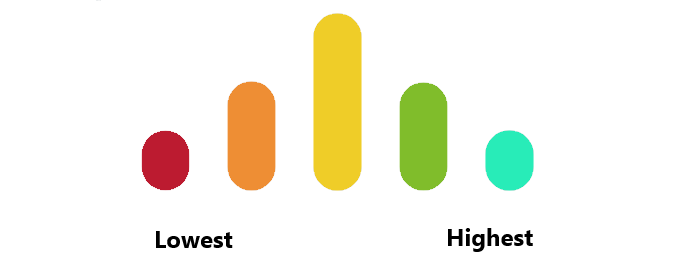
\includegraphics[scale=0.8]{images/colors.png}
    \caption{Colori del valore sociale}
    \label{fig:colours}
\end{figure}

Yup permette anche la visualizzazione del valore (sociale) di un contenuto, in base ai voti che ha ricevuto e a patto che sia stato votato almeno una volta, in relazione a tutti i contenuti che sono stati votati in una determinata categoria. Questo viene fatto tramite l'utilizzo di cinque colori in accordo con quelli dei cinque rating possibili.
\begin{itemize}
    \item \textbf{Verde:} top 20\%
    \item \textbf{Verde Giallastro:} 20\% - 40\%
    \item \textbf{Giallo:} 40\% - 60\%
    \item \textbf{Arancione:} 60\% - 80\%
    \item \textbf{Rosso:} 80\% - 100\%
\end{itemize}
I colori dei rating sono mostrati in Figura \ref{fig:colours}.

I voti negativi tendono a far diventare il colore di un contenuto più rosso e quelli positivi più verde. E' importante specificare come un contenuto potrebbe avere differenti colorazioni al variare della categoria. Per esempio, un tweet potrebbe aver ricevuto valutazioni estremamente positive per la categoria \textbf{Smart} ma valutazioni intermedie o negative per la categoria \textbf{Funny}.

\subsection{Integrazioni}
L'integrazione con l'estensione di YUP, intesa come la possibilità di esprimere un voto tramite l'\textbf{Overlay} piuttosto che l'estensione, è al momento disponibile solo su alcune piattaforme, principalmente riguardanti i Social Media:

\begin{itemize}
    \item \textbf{Twitter}
    \item \textbf{Youtube}
    \item \textbf{Reddit}
    \item \textbf{Google Maps}
\end{itemize}

Twitter costituisce un caso a parte poichè è attualmente l'unica piattaforma ad essere integrata anche tramite \textbf{OAuth}, ovvero è possibile registrarsi su Yup e verificare il proprio account tramite quello di Twitter.
Le prossime piattaforme per cui è programmata l'integrazione sono quelle relative al mercato di NFT quali \textbf{SuperRare}, \textbf{Audius} e \textbf{Rarible}. Al momento supportano comunque almeno l'\textbf{Action Tracking}, ovvero l'estensione registra i Like espressi su queste piattaforme e genera un corrispondente rating di 3/5 in categoria "Like", cosa che già avviene nelle piattaforme che supportano l'integrazione.

\section{Yup protocol}
Lo Yup Protocol è un protocollo di consenso sociale promosso ed incentivato da un'economia che si basa sulle opinioni degli utenti che fanno parte della rete, dove quest'ultima esiste all'interno del \textit{framework} del protocollo stesso.
Il protocollo facilita la misura, l'acquisizione e lo scambio di capitale sociale assicurando trasparenza e anonimità, anche se vedremo come quest'ultima non sempre sia garantita.
\\
Nello specifico il protocollo garantisce:
\begin{enumerate}
    \item \textit{Trasparenza}
    \item \textit{Monetizzazione equa e diretta} di contenuti e opinioni
    \item \textit{Identità digitali}
    \item \textit{Codici di condotta community-driven}
    \item \textit{Governance} basata sull'influenza
    \item \textit{Equa distribuzione} dei profitti pubblicitari
\end{enumerate}

Nelle sezioni successive vedremo come viene calcolato il peso che un utente e le sue azioni hanno all'interno della rete (\textbf{Influenza}), riservando opportuna attenzione anche a come sono definiti e calcolati i singoli parametri che contribuiscono a tale valore (\textbf{Age}, \textbf{Activity}, \textbf{Social Level} e \textbf{Boost}). Tratteremo inoltre alcuni aspetti tecnici del meccanismo delle ricompense e concluderemo con la trattazione dello strumento (\textbf{EOS-ETH Bridge} che permette a Yup di essere una piattaforma cross-chain e cross-platform.

\subsection{Influenza}
L'\textbf{Influenza} è una metrica, misurata nel range $0-100$, utilizzata come fondamento della \textit{governance} di rete ma anche per regolare la distribuzione dei token ricompensa.
Può essere definita come una rappresentazione del valore sociale di un utente: più alto è questo valore più peso avranno le sue opinioni. L'\textbf{Influenza} varia in base a quattro componenti che elenchiamo:

\begin{itemize}
    \item \textbf{Age (A)}
    \item \textbf{Activity (a)}
    \item \textbf{Social Level (s)}
    \item \textbf{Boost (b)}
\end{itemize}

Il suo valore è calcolato dal protocollo, per ogni utente, secondo l'equazione \ref{eq: influence_eq}:

\begin{equation}\label{eq: influence_eq}
    I = \beta\textsubscript{1}\sqrt{A} + \beta\textsubscript{2}\sqrt{a} + \beta\textsubscript{3}\sqrt{s} + b
\end{equation}

Dove i $\beta\textsubscript{i}$ sono delle costanti che nella documentazione non vengono specificate/spiegate. 
Di seguito, entreremo nel dettaglio dei singoli componenti: \textbf{Age}, \textbf{Activity}, \textbf{Social Level}, ed infine \textbf{Boost}.

\subsubsection{Age}
I token mantenuti da un account sono rappresentati dall'\textbf{Age} in un modo che si differenzia dal semplice \textit{staking - unstaking}. Infatti, oltre che considerare la quantità di token, viene tenuto in considerazione anche da quanto tempo l'utente ne è in possesso. Ne conseguono i seguenti vantaggi:
\begin{enumerate}
    \item Riflette l'impegno di un individuo all'interno della rete, impedendo che nuovi utenti possano incrementare in maniera significativa la propria influenza semplicemente comprando grandi quantità di token in un breve periodo
    \item Permette al protocollo di sostituire completamente il processo di \textit{staking - unstaking}, senza rinunciare a sicurezza a stabilità.
    \item Rende il tempo una vera e propria risorsa per gli utenti
\end{enumerate}

Definiamo questo parametro nell'equazione \ref{eq: age_eq}:

\begin{equation}\label{eq: age_eq}
    A = \sum\limits_{i=1}^nY\textsubscript{i}t\textsubscript{i}
\end{equation}

Dove $Y\textsubscript{i}$ rappresenta il \textit{token value} di una transazione che assegna dei token ad un utente e $t\textsubscript{i}$ il tempo trascorso dalla sua attuazione. 
\\
Notiamo come si dia importanza al tempo trascorso dal momento in cui un utente ottiene dei token.
% corretto commento di Andrea

\subsubsection{Activity}
L'\textbf{Activity} è una misurazione dell'attività e dell'impegno di un utente all'interno della rete. Per determinarla consideriamo i token YUP ottenuti dall'utente come ricompensa, sia essa per creazione o cura di contenuti, escludendo quindi quelli semplicemente acquistati. Esprimiamo l'Activity con l'equazione \ref{eq: activity_eq},

\begin{equation}\label{eq: activity_eq}
    a = \sum\limits_{i=1}^nR\textsubscript{u,i}
\end{equation}

dove $R\textsubscript{u,i}$ rappresenta le ricompense ricevute da uno specifico utente $u$ per un'azione $i$.
\\
E' importante notare come questo parametro non sia influenzato né dall'\textbf{Age} né dal bilancio dei token posseduti. In questo modo si evita che esso cambi nel momento in cui un utente trasferisce i token guadagnati. Inoltre per scoraggiare un'eccessiva attività priva di qualità col solo scopo di aumentare il valore  di activity, viene imposto un limite di 10 azioni giornaliere al conteggio dell'activity. Sarà ancora possibile effettuare delle azioni dopo le prime 10, tuttavia avranno un impatto nullo o marginale.

\subsubsection{Social Level}
Il \textbf{Social Level}, indicato con $\Bar{s}$ (\ref{eq: social_level_eq}), è un \textit{rank} numerico caratteristico di ogni account che viene determinato in base a tutti gli altri utenti (indirizzi) presenti nel network. Ogni account mantiene una lista, ordinata in un modo specifico che può modificare, di tutti gli altri utenti.
Definiamo questo parametro come segue,
% corretto commento di Andrea: [DOCUMENTAZIONE NON CHIARA, NON SIAMO SICURI DI QUESTO SOCIAL LEVEL]

\begin{equation}\label{eq: social_level_eq}
  \Bar{s} = \sum\limits_{i=1} \frac{s\textsubscript{i}*(\log (w\textsubscript{i}) + 1)}{\sqrt[5]{e\textsubscript{p}}}
\end{equation}

dove,
\begin{itemize}
    \item \textit{w (Weight)}: è un peso relativo ad un \textbf{ordine utente (UO)} ed è calcolato in base al livello dell'utente nell' \textbf{ordine aggregato (AO)} del blocco precedente (più qualche piccolo aggiustamento). Si veda Figura \ref{fig: social_table}.
    % corretto commento di Andrea [DA CHIEDERE: parte poco chiara su documentazione]
    \item \textit{e (Error)}: è una misura che dipende dalla relazione tra la lista mantenuta dall'utente e quella aggregata. Incentiva gli utenti ad effettuare un ordinamento corretto, poiché nel caso questo sia errato ne consegue una importante riduzione del loro livello sociale.
\end{itemize}

L'errore $e$ (\ref{eq: error_eq} viene espresso come la somma dei quadrati delle differenze tra il valore di ciascun elemento della lista $r$ e il corrispettivo \textit{rank} medio dell'account $\mu$,

\begin{equation}\label{eq: error_eq}
    e = \sum\limits_{i=1} (r\textsubscript{i} - \mu\textsubscript{i})^2
\end{equation}

Possiamo meglio comprendere il modo in cui funzionano i due diversi ordinamenti (AO e UO) tramite l'analisi delle Figura \ref{fig: social_table} e \ref{fig: social_simplified}.

\begin{figure}[h!]
    \centering
    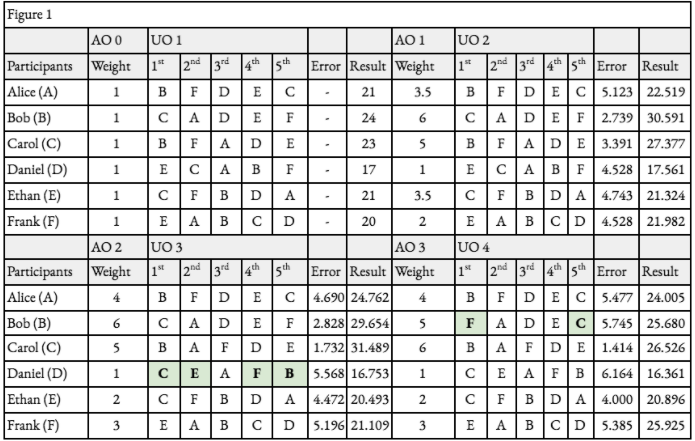
\includegraphics[width=\textwidth]{sociale_level}
    \caption{Ordinamento del Social Level}
    \label{fig: social_table}
\end{figure}

Alice (A), Bob (B), Carol (C), Daniel (D), Ethan (E), e Frank (F) sono i partecipanti di una rete con lo stesso protocollo di quello presentato. Questi utenti si elencano a vicenda nel "blocco di genesi" della piattaforma che utilizzano, dal più alto al più basso. Osserviamo i voti da loro espressi nei round 1, 2, 3, e 4 (UO) nella Figura \ref{fig: social_table}. Nel primo round il loro peso all'interno del network è uniforme mentre nel round 2 e nei successivi questo, e di conseguenza l'ordine, cambia.
Nel round 2 (UO 2) abbiamo i seguenti nuovi pesi per i sei account considerati: (A, 3.5), (B, 6), (C, 5), (D, 1) e i corrispondenti livelli sociali osservabili nella colonna \textit{Result} dell'immagine. Bob è quindi l'utente con più influenza e Daniel quello più basso. Nel round 3, Daniel tenta di incrementare l'influenza di Carol e decrementare quella di Bob mettendo la prima al vertice della sua lista ed i secondo in ultima posizione. Questo incrementa considerevolmente l'errore di Daniel (da 4.528 a 5.568) ma  fa andare con successo Carol al primo posto della lista (Carol UO 3 Result: 31.489), diventando prima in AO 3. Bob, con l'obiettivo di riprendersi la sua posizione, ordina Carol in ultima posizione nel round. Questo riduce la differenza tra Carol e Bob così come quella tra Carol e gli altri utenti. Tuttavia incrementa notevolmente l'errore di Bob (da 2.828 a 5.745) che fa diminuire il suo punteggio finale (Bob UO 4 Result: 25.680) e previene il suo tentativo di superare Carol.

\begin{figure}[h!]
    \centering
    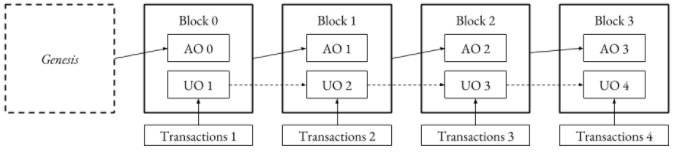
\includegraphics[width=\textwidth]{social_level_order}
    \caption{Ordinamento semplificato del Social Level}
    \label{fig: social_simplified}
\end{figure}


Se volessimo vedere quanto appena trattato in maniera più semplice possiamo osservare la Figura \ref{fig: social_simplified}. Osserviamo come l'ordine aggregato (AO) sia relativo ad ogni blocco e derivi da informazioni contenute nel blocco precedente, nello specifico dal blocco di genesi, in cui tutti i partecipanti hanno il medesimo peso, quando ci troviamo nella prima fase. L'ordine specifico di un utente (UO) invece, in assenza di transazioni che lo modifichino, rimane invariato tra un blocco e l'altro.

\subsubsection{Boost (Burning Mechanism)}
Con lo scopo di mantenere la fornitura di Yup tokens in distribuzione e aumentare la richiesta di questi ultimi, il protocollo fornisce un meccanismo definito come \textbf{Burning Mechanism}. Questo permette ad un account di "bruciare" permanentemente token posseduti per un temporaneo incremento della sua \textit{Influenza} (I) su una specifica azione da lui eseguita. Il numero di token che un account può investire con questo proposito è limitato.
Il \textbf{Boost} viene definito come nell'equazione \ref{eq: boost_eq},

\begin{equation}\label{eq: boost_eq}
    b = \sigma Y\textsubscript{burn,u}
\end{equation}

dove $\sigma$ è un \textbf{boost multiplier}.

\subsection{Meccanismo delle ricompense}
Il meccanismo di \textit{reward} dei token è una parte fondamentale del protocollo, in quanto si occupa della generazione di nuovi token e della loro successiva distribuzione. Esistono tre tipi di ricompense:

\begin{itemize}
    \item \textbf{Ricompense creatore} 
    \item \textbf{Ricompense curatore} 
    \item \textbf{Ricompense LQ:} destinate ai Liqiduity Provider
\end{itemize}

Gran parte dei token generati vengono distribuiti agli autori di contenuti in maniera proporzionale alle valutazioni che essi hanno ricevuto dalla \textit{community}. Questa frazione prende il nome di \textbf{creation allocation}. Tuttavia prima di darne una espressione in formule matematiche è necessario definire altri due elementi.
\\
\\
Nell'equazione \ref{eq: action_value} indichiamo con $V\textsubscript{h}$ il valore di una determinata azione che viene effettuata nella rete tramite l'interazione con il protocollo. Questa è espressa come il rapporto tra l'Influenza dell'azione e quella totale delle azioni eseguite sulla rete in un determinato periodo di tempo. Dove con Influenza di un'azione indichiamo semplicemente il valore I, precedentemente descritto, dell'utente che la effettua. 

\begin{equation}\label{eq: action_value}
    V\textsubscript{h} = \frac{I\textsubscript{i}}{I\textsubscript{i,t}} Y\textsubscript{c,t}
\end{equation}

Nell'equazione \ref{eq: content_value} indichiamo con $R\textsubscript{i}$, che prende il nome di \textbf{creation reward}, il valore in token di un contenuto, espresso come sommatoria dei valori delle azioni $V\textsubscript{j}$ eseguite per la creazione di quest'ultimo.

\begin{equation}\label{eq: content_value}
    R\textsubscript{i} = \sum\limits_{j=1}^m V\textsubscript{j}
\end{equation}


Adesso possiamo finalmente dare una definizione di \textbf{creation allocation} (\ref{eq: creation_allocation}). La definiamo, in relazione ad un determinato periodo di tempo $t$, come la sommatoria di tutte le corrispondenti \textbf{creation reward}.


\begin{equation}\label{eq: creation_allocation}
    Y\textsubscript{c,t} = \sum\limits_{i=1}^n R\textsubscript{i}
\end{equation}

\subsubsection{Ricompense Creatori e Curatori}
Definiamo la ricompensa di un \textbf{Creatore} $R\textsubscript{c}$ (\ref{eq: creator_reward}) come la porzione della ricompensa di un contenuto assegnata al creatore di quest'ultimo.
Sotto qualsiasi circostanza il creatore di un contenuto riceverà almeno il $50\%$ della ricompensa, mentre la parte rimanente viene divisa, in base all'influenza, tra il creatore e tutti i curatori che hanno contribuito al contenuto.
Definiamo $I\textsubscript{c}$ come l'influenza del creatore durante il periodo che intercorre dal momento della creazione e $I\textsubscript{pool,t}$ come la somma totale dell'Influenza di tutti i curatori che hanno votato il contenuto. In poche parole la porzione della seconda metà assegnata al creatore dipende dal rapporto tra la sua influenza e quella della \textit{pool}.
Possiamo ora esprimere $R\textsubscript{c}$ come,


\begin{equation}\label{eq: creator_reward}
    R\textsubscript{c} = R\textsubscript{i}\left(\frac{1 + \frac{I\textsubscript{c}}{I\textsubscript{pool,t}}}{2}\right)
\end{equation}
\\
\\
Ogni curatore riceve delle ricompense tenendo conto esclusivamente dei voti a loro successivi, i precedenti vengono pertanto ignorati. In questo modo si ricompensano maggiormente i curatori che hanno espresso una valutazione corretta sin da subito rispetto a coloro che arrivano in ritardo e che, in certi casi, potrebbero esprimere un'opinione condizionati dai voti già espressi. 
Definiamo la ricompensa di un \textbf{Curatore} $R\textsubscript{q}$ (\ref{eq: curator_reward}) come,

\begin{equation}\label{eq: curator_reward}
   R\textsubscript{q} = (\frac{1 - \frac{I\textsubscript{c}}{I\textsubscript{pool,t}}}{2}) \sum\limits_{j=1}^n (\frac{V\textsubscript{q}}{V\textsubscript{h,j}}) V\textsubscript{j}
\end{equation}


Dove $V\textsubscript{q}$ è il valore assegnato all'azione del curatore. $V\textsubscript{j}$ è un'azione $j$ a lui successiva mentre $V\textsubscript{h,j}$ rappresenta la somma dei valori delle azioni precedenti a $V\textsubscript{j}$.
\\
\\
Infine, indichiamo come ricompense LQ quelle destinate ad utenti che forniscono liquidità nella pool YUP-ETH di Uniswap. Queste sono proporzionali al numero di token YUP-ETH LQ messi in stake su \textit{Yup Racing}\footnote{https://www.yup.finance/}. Nella documentazione non vengono descritte formule relative al calcolo di quest'ultimo tipo di ricompense.
% corretto commento di Andrea [DA CHIEDERE: se devo spostare parte LQ qui]
% corretto commento di Andrea [DA CHIEDERE: Yup Racing non è citato prima perchè non sappiamo nulla se non che serva per lo stake di YUP-ETH]

\subsection{EOS-ETH Bridge}
Essendo Yup una piattaforma che si basa sull'utilizzo di due blockchain differenti, ne consegue la necessità di un meccanismo che permetta una interazione tra queste ultime. Questo ruolo viene ricoperto dallo \textbf{Yup Bridge}. La funzionalità è quella di rendere possibile il trasferimento di token tra le due blockchain. La modalità con cui i token vengono trasferiti tra le due blockchain prende il nome di \textbf{mint - burn}, i token non vengono effettivamente spostati bensì eliminati (burnt) su una blockchain e successivamente ne viene creato un quantitativo corrispondente sull'altra. Il servizio del \textbf{Bridge} è offerto da terzi e comporta per ogni spostamento di token il pagamento di una tassa, corrispondente ad una porzione degli YUP di cui si intende effettuare la migrazione. Il valore di questa tassa è direttamente correlato con il \textbf{gas} di Ethereum.

\section{Yup token}
Il token Yup è progettato per essere un \textit{crypto-asset} fruibile che permetta di creare un'economia sociale fondata sull'attività della \textit{community}. Esiste una versione del token sia su Ethereum che su EOS, il valore varia in base alla liquidità presente su quella specifica blockchain. 
Il token raggiunge i seguenti scopi:

\begin{itemize}
    \item \textbf{Incentivazione della partecipazione:} poichè utilizzati come ricompensa,
    \item \textbf{Governance:} in quanto utilizzato per governare il protocollo,
    \item \textbf{Incentivazione della liquidità:} i fornitori di liquidità ottengono Yup tokens come ricompensa,
\end{itemize}

Coloro che desiderano fornire liquidità per il protocollo devono aggiungere alla pool di Uniswap un volume equivalente di token ETH e token YUP. Per ottenere questi ultimi su Ethereum è sufficiente acquistarli in un exchange della blockchain oppure trasferire da EOS quelli guadagnati come ricompense curatore per l'utilizzo della piattaforma. Una volta inserita liquidità vengono ricompensati con dei token YUP-ETH Uniswap LP, questi ultimi attestano la loro percentuale di ownership della pool su Uniswap. Per concludere è necessario migrare questi ultimi su EOS e metterli in stake su Yup Racing. A questo punto si iniziano a ricevere token Yup, in proporzione alla liquidità fornita.
\\
\\
Nuovi token vengono creati secondo un programma prefissato per mezzo del \textit{token reward mechanicsm}, lo stesso meccanismo che si occupa anche della loro distribuzione.
\\
Il token di cui abbiamo appena parlato è stato introdotto nel protocollo una volta terminata la fase di \textbf{Beta testing} verso Settembre/Ottobre 2019. Precedentemente veniva utilizzato un altro token, indicato con \textbf{YUPX}, privo di valore il cui unico scopo era eseguire dei test sul corretto funzionamento del protocollo. Una volta conclusa la fase iniziale del progetto tutti gli utenti che vi avevano preso parte hanno ricevuto token YUP in rapporto 1 a 1 con i YUPX posseduti.

\section{Scopo del Tirocinio}
Le piattaforme Social Media basate su blockchain rappresentano oggi una valida alternativa alle soluzioni centralizzate, ed il meccanismo di reward risulta essere un ottimo metodo per incentivare la partecipazione degli utenti.
Lo scopo di questa tesi è far luce sul funzionamento della dApp di Yup, che risulta essere attualmente, una delle dApp sociali più utilizzate, con circa 6.000 utenti attivi al giorno\footnote{https://www.dapp.com/app/yup}. Ci siamo concentrati sulle possibili caratteristiche di un successo così importante, andando ad analizzare dettagliatamente il protocollo ed il meccanismo di reward, ed infine analizzando l'attività degli utenti. Nello specifico, abbiamo analizzato l'ambito sociale ed economico della piattaforma, quest'ultimo particolarmente importante nell'incentivare l'utilizzo della piattaforma stessa. Tra l'altro Yup si discosta proprio in questo ambito dalle numerose concorrenti anche solo per il valore del token che si riceve come ricompensa. Per esempio, durante \textit{Gennaio-Marzo 2021}, ha avuto un minimo di \textit{\euro1.28} ed un massimo di \textit{\euro5.85}. Se lo confrontiamo per esempio con i token utilizzati da social dApp concorrenti vediamo che: la moneta utilizzata su Hive, quindi da PeakD e Hive Blog, non ha mai superato nemmeno il valore di \textit{\euro1}, oppure quella utilizzata da Steemit, STEEM, solo recentemente, e per pochi giorni, ha superato il valore di \textit{\euro1}.


\subsection{Fase di studio}
\label{fasestudio_marker}
Nel protocollo di Yup sono presenti, in accordo con l'explorer utilizzato, 51 azioni differenti. Le elenchiamo di seguito suddivise per categoria e daremo una descrizione dettagliata esclusivamente di quelle più utilizzate e/o di cui è stato possibile comprenderne la funzionalità grazie al nome, al corpo JSON o tramite alcuni test effettuati durante la fase di analisi.

\begin{table}[t]
    \centering
    \caption{Azioni ambito \textbf{sociale}}
    \begin{tabular}{|l|l|l|l|}
    \hline
    $\bullet$ createcomv2 & $\bullet$ createvotev2 & $\bullet$ createvotev3 & $\bullet$ createvotev4 \\
    \hline
    $\bullet$ deletecom & $\bullet$ deletevote & $\bullet$ editacct & $\bullet$ editacct2 \\
    \hline
    $\bullet$ editvotev2 & $\bullet$ follow & $\bullet$ unfollow & $\bullet$ postvote \\
    \hline
    $\bullet$ postvotev2 & $\bullet$ postvotev3 & $\bullet$ postvotev4 \\
    \cline{1-3}
    \end{tabular}
    \label{tab: social_actions}
\end{table}

\begin{table}[t]
    \centering
    \caption{Azioni ambito \textbf{economico}}
    \begin{tabular}{|l|l|l|l|}
    \hline
    $\bullet$ claimcrrwds & $\bullet$ claimcurwds & $\bullet$ claimlqrwds2 & $\bullet$ stakelq \\
    \hline
    $\bullet$ unstakelq \\
    \cline{1-1}
    \end{tabular}
    \label{tab: economy_actions}
\end{table}
\clearpage

\begin{table}[t]
    \centering
    \caption{Azioni di \textbf{sistema}}
    \begin{tabular}{|l|l|l|l|}
    \hline
    $\bullet$ addblacklist & $\bullet$ addnblcklist & $\bullet$ createacct & $\bullet$ createcat \\
    \hline
    $\bullet$ getactivity & $\bullet$ getage & $\bullet$ getinfl & $\bullet$ getivlpool \\
    \hline
    $\bullet$ logacctv2 & $\bullet$ logactivity & $\bullet$ logage & $\bullet$ loggetage \\
    \hline
    $\bullet$ login & $\bullet$ loginfluence & $\bullet$ loguintval & $\bullet$ rmblacklist \\
    \hline
    \end{tabular}
    \label{tab: system_actions}
\end{table}

\begin{table}[t]
    \centering
    \caption{Azioni \textbf{sconosciute}}
    \begin{tabular}{|l|l|l|l|}
    \hline
    $\bullet$ claimtmrwds & $\bullet$ claimtrrwds & $\bullet$ delactusg & $\bullet$ dellqivls \\
    \hline
    $\bullet$ initvotecks & $\bullet$ logdouble & $\bullet$ logdoubleval & $\bullet$ noop \\
    \hline
    $\bullet$ processivlv3 & $\bullet$ processlqivl & $\bullet$ rmactusage & $\bullet$ setvotecks \\
    \hline
    $\bullet$ updatelstivl & $\bullet$ updlstlqivl & $\bullet$ vmcomp \\
    \cline{1-3}
    \end{tabular}
    \label{tab: unknown_actions}
\end{table}

\subsubsection{postvote}
L'azione di \textbf{postvote} (di cui possiamo trovare multiple versioni: postvote, postvotev2, postvotev3 e postvotev4) corrisponde alla votazione di un contenuto, non precedentemente valutato, da parte di un utente.
\\
Per l'esecuzione della azione sono necessari due attori e di conseguenza due chiavi private, quella di \textbf{yupcreators1} e dell'utente che ha espresso l'opinione. Troviamo queste informazioni nel campo \textbf{authorization} della postvote.
Le informazioni relative al voto sono invece presenti nel campo \textbf{data}. Elenchiamo le più importanti:

\begin{itemize}
    \item \textbf{caption:} link completo del contenuto votato
    \item \textbf{voter:} il nome EOS dell'account del votatore
    \item \textbf{category:} la categoria in cui è stato espresso il voto
    \item \textbf{like:} booleano settato 1 o 0, rispettivamente se il voto è positivo o negativo
    \item \textbf{rating:} un intero che indica l'intensità del voto in un range 1-3 se positivo e 1-2 se negativo
\end{itemize}

Ricordiamo quanto detto in Sezione \ref{voti_section}, ovvero che un voto viene misurato in una scala che va da 1/5 a 5/5. Le valutazioni 1/5 e 2/5 sono negative le restanti sono positive. Il modo in cui questi valori sono rappresentati con i parametri \textbf{like} e \textbf{rating} elencati sopra è il seguente: se like è settato a 0, quindi voto negativo, il campo rating potrà presentarsi con valore 1 o 2, rispettivamente l'equivalente di 1/5 e 2/5, se invece like è settato a 1, quindi voto positivo, potremo trovare nel campo rating il valore 1, 2 o 3, rispettivamente 3/5, 4/5 e 5/5.
\\
\\
L'unica differenza che è stato possibile osservare tra le varie versione di postvote è l'aggiunta di due parametri nel campo \textbf{data} nelle versioni v3 e v4:

\begin{itemize}
    \item \textbf{ram\_payer:} sempre yupcreators1
    \item \textbf{postid:} l'id con cui il contenuto viene salvato nel database di Yup
\end{itemize}

\subsubsection{createvote}
L'azione di \textbf{createvote} (di cui possiamo trovare le seguenti versioni: createvotev2, createvotev3 e createvotev4) corrisponde alla votazione di un contenuto già precedentemente valutato da un utente.
I campi in cui troviamo le informazioni relative alle autorizzazioni necessarie per la sua esecuzione e quelle relative al voto sono le stesse elencate precedentemente per la postvote. In questo caso troviamo, nel campo \textbf{authorization}, solo un attore che rappresenta l'utente. Questo vale solo per le versioni fino alla v3, infatti nel caso specifico della v4 compare anche un campo che indica anche yupcreators1 come attore.
\\
Per quanto riguarda le informazioni relative al voto, i parametri presenti nel campo \textbf{data} sono esattamente gli stessi che avevamo precedentemente elencato per postvote e postvotev2. L'unica differenza è che al posto del link del contenuto troviamo semplicemente l'id con cui è identificato nel database di Yup ("postid").

\subsubsection{claimcurwds}
L'azione di \textbf{claimcurwds} è relativa alla distribuzione delle ricompense per gli utenti in qualità di curatori. In questa sezione non discuteremo le claim di cui non siamo riusciti a comprendere la natura (\textbf{claimtmrwds} e \textbf{claimtrrwds}). Il corpo dell'azione presenta, nel campo \textbf{data}, un parametro che specifica il voteid, che permette di risalire anche al postid del contenuto, a cui fanno riferimento le ricompense assegnate. 
\\
Alcune variante della \textbf{claimcurwds} sono la \textbf{claimcrrwds} e la \textbf{claimlqrwds2}, rispettivamente relative alle ricompense creatori e a quelle LQ. La calimcrrwds ha come destinatario sempre yupcreators1 e contiene nel campo \textbf{data} il postid del contenuto creato. La claimlqrwds2 invece mantiene in tale campo semplicemente l'eosname dell'utente LQ a cui spettano le ricompense in questione.
\\
\\
Tramite lo studio effettuato sulla blockchain è stato possibile individuare ulteriori tipi di azioni che non erano presenti nella lista dell'explorer precedentemente mostrata. Elenchiamo queste ultime nella Tabella \ref{tab: appendix_actions} in Appendice A a pag. \pageref{appendix_marker}. Delle azioni mostrate in Appendice siamo riusciti a comprendere la funzionalità della \textbf{transfer}, la quale sembrerebbe propria di EOS per spostamenti di token e risorse.

\subsubsection{transfer}
Di seguito diamo una descrizione dei principali parametri individuati all'interno del campo \textbf{data} dell'azione in questione.

\begin{itemize}
    \item \textbf{from:} il mittente (yupyupyupyup nel caso di ricompense o il nome di un utente altrimenti)
    \item \textbf{to:} il nome EOS dell'utente
    \item \textbf{quantity:} il numero di token inviati
    \item \textbf{memo:} specifica la natura del trasferimento e presenta cinque possibilità: "Yup Creators Rewards", "Yup LQ Rewards", "Yup Extension Transfer", "Bridge Fee" e un indirizzo Ethereum. Rispettivamente sono relative a ricompense creatore, a ricompense liquity provider, al trasferimento utente-utente tramite l'estensione, al pagamento della tassa per il Bridge oppure al trasferimento su Ethereum dei propri token.
\end{itemize}

Durante le fase di studio del protocollo, abbiamo analizzato il meccanismo di ricompensa e gli Smart Contract utilizzati, focalizzandoci su quello principale (yupyupyupyup). 
Gli Smart Contract di Yup su EOS si differenziano, oltre a quello principale su cui ci siamo concentrati, da quelli relativi ai token, token.yup e lptoken.yup rispettivamente per il token ricompensa Yup ed il token YUP-ETH dei Liquidity Provider, a quelli relativi al servizio del Bridge, bridge.yup e lpbridge.yup rispettivamente per il Bridge relativo ai token Yup e per il Bridge relativo ai token YUP-ETH.
% commento Andrea [DA CHIEDERE: azioni/transazioni sono proprie di EOSIO più che di EOS, dove aggiungerne spiegazione]

Non tutte le azioni della lista sono state poi ritrovate nell'attività dello Smart Contract.
Pertanto, effettuando una intersezione ed un'unione dei due gruppi di azioni trovati, otteniamo i seguenti dati:

\begin{itemize}
    \item \textbf{AZIONI LISTA:} 51
    \item \textbf{AZIONI TROVATE:} 192
    \item \textbf{IN COMUNE:} 46
    \item \textbf{TOTALE:} 197
\end{itemize}

Pertanto abbiamo 5 azioni della lista che non sono state ritrovate nel protocollo: \textit{getactivity}, \textit{getage}, \textit{loggetage}, \textit{rmactusage} e \textit{vmcomp}. Dove le prime due iniziano ad essere utilizzate a partire dal \textit{21 Marzo 2021}, mentre le rimanenti non sono ancora mai state utilizzate. Abbiamo 146 azioni (Tabella \ref{tab: appendix_actions} in Appendice A a pag. \pageref{appendix_marker}) individuate durante la fase di analisi dei dati della blockchain che non vengono ritrovate nella lista dell'explorer.
\\
\\

\subsection{Fase di download}
Per scaricare i dati dalla blockchain è stato necessario recuperare i nomi dei vari Smart Contracts dalla documentazione di Yup e successivamente utilizzare l'endpoint \textit{Get Actions} delle API offerte da \textit{eosflare.io}, effettuando un numero di richieste in accordo con il limit rate imposto (\textit{100/Min}). E' stato invece possibile scaricare le informazioni relative agli account Yup esistenti grazie alle API (endpoint: \textit{/levels}) descritte nella documentazione.
Durante la fase di download, abbiamo collezionato le informazioni relative a tutte le azioni eseguite su Yup. Abbiamo poi recuperato le informazioni relative agli accounts registrati su Yup ed infine quelle relative ai singoli contributi sociali, ovvero i vari contenuti votati.
%I programmi utilizzati per fare quanto detto sopra sono stati realizzati in linguaggio Python. E' stata utilizzata una libreria esterna (\textit{ijson}) per gestire le elevate dimensioni del JSON risultate dal download dello storico di tutte le azioni.

\subsection{Fase di analisi}
Durante la fase di analisi ci siamo concentrati principalmente nell'analisi economica e sociale della piattaforma, andando a valutare l'attività degli utenti. In dettaglio, abbiamo osservato vari aspetti del protocollo, tra cui l'utilizzo delle varie azioni, l'attività in termini di utenza, le varie piattaforme sociali coinvolte, ecc. Nel Capitolo \ref{analisi_marker}, sono riportate tutte le analisi effettuate e le considerazioni sui risultati ottenuti.
%\\
%\\
%In base alle analisi effettuate abbiamo appurato l'esistenza di \textit{16.484} account Yup, di questi solo per \textit{10.914} è stato possibile ritrovare una corrispondente azione di creazione account nel protocollo. Considerando solo il periodo successivo alla conclusione della fase di Beta (\textit{6 Ottobre 2020 - Febbraio 2021}), risulta una media di circa \textit{700} utenti mensili socialmente attivi, ovvero che hanno effettuato almeno un'azione in ambito sociale in quel mese. Di questi è stato osservato un picco particolarmente alto nel mese di Settembre, specificamente tra il 23 e 24 del mese. Queste ultime considerazioni sono relative ai soli account non-Mirror, tuttavia nel capitolo dedicato alla fase di analisi tratteremo anche quelle che tengono in considerazione gli account di sistema.
%\\
%\\
%Restando in ambito sociale abbiamo individuato 1.884 piattaforme diverse che hanno ricevuto almeno un voto. Tra queste dominano tre delle quattro piattaforme integrate (in ordine Twitter, Youtube e Reddit), anche se è possibile notare una notevole presenza di quelle ad NFT. Vedremo come la maggior parte dei profili o gruppi votati all'interno di tali piattaforme trattino argomenti legati al mondo cripto.
%\\
%\\
%Spostandoci infine sull'ambito economico abbiamo analizzato il funzionamento del meccanismo di ricompense e la distribuzione dei token tra i vari utenti. Nel primo caso è stato notato come quelle destinate ai Creatori non vengano distribuite agli account Mirror corrispondenti bensì accumulate sull'account \textbf{yupcreators1}, apparentemente per una futura distribuzione quando più Creatori riscatteranno tali account o si iscriveranno alla piattaforma. Nel secondo è stato possibile osservare come gli utenti che hanno riscosso o possiedono più token siano, nella maggior pate dei casi, utenti che, oltre ad utilizzare il servizio, forniscono liquidità su Uniswap.
%\\
%\\
%\subsubsection{Introduzione ai grafici}
%Osserveremo nel dettaglio i risultati di questa fase nell'apposito capitolo (\textbf{Chapter 5: ANALISI}). Vedremo alcuni grafici, opportunamente commentati, che ci aiutano a comprendere i dati raccolti. Questi ultimi rappresentano in certi casi un'analisi della distribuzione dei dati in relazione a determinate categorie, ed in altri un'analisi temporale, sia essa effettuata su base mensile o giornaliera. In quasi tutti i casi effettueremo una distinzione tra account reali (non-Mirror) e di sistema (Mirror). Infine, nel caso specifico di analisi distributive, rappresenteremo solo una top 10 dei dati per motivi di ordine e comprensione, includeremo tutti quelli restanti nella categoria \textit{others}.
